% Chapter 9
\section{\texorpdfstring{Introduction to Self-Organizing Networks\\and Unsupervised Learning}{Introduction to Self-Organizing Networks and Unsupervised Learning}}\label{chap:som}
\graphicspath{{assets/lec5/}}

\begin{tcolorbox}[summarybox,title={Learning Outcomes}]
\begin{itemize}
    \item Describe how competitive learning, cooperation, and annealing interact in SOM training.
    \item Monitor SOM quality via quantization/topographic errors and interpret U-Matrices.
    \item Connect SOMs to broader unsupervised techniques (clustering, dimensionality reduction) and know when to use each.
\end{itemize}
\end{tcolorbox}

\Cref{chap:rbf} offered a nonlinearity that stays close to linear algebra (basis expansion + linear solve). Here we switch to an unsupervised lens: self-organizing maps discover prototypes and organize them on a lattice without labels. The roadmap in \Cref{fig:roadmap} highlights this as the competitive/unsupervised branch.

\begin{tcolorbox}[summarybox,title={Design motif}]
Competition plus cooperation: pick a winner, then let its neighbors learn too, so the map becomes both a clustering device and a visualization.
\end{tcolorbox}

\begin{tcolorbox}[summarybox,title={Tiny numeric step (online update)}]
Input \(\mathbf{x}=[0.2,0.8]\), two map units with weights \(\mathbf{w}_1=[0.1,0.9]\), \(\mathbf{w}_2=[0.7,0.3]\), coordinates \(\mathbf{r}_1=[0,0]\), \(\mathbf{r}_2=[1,0]\), \(\alpha=0.5\), \(\sigma=1\). BMU \(c=1\) (closest to \(\mathbf{x}\)). Neighborhoods: \(h_{11}=1\), \(h_{21}=\exp(-1/2)\approx 0.607\). Updates:
\[
\mathbf{w}_1\leftarrow [0.15,\,0.85],\quad
\mathbf{w}_2\leftarrow [0.548,\,0.452].
\]
Even the neighbor moves toward \(\mathbf{x}\), illustrating cooperation.
\end{tcolorbox}

In this chapter, we begin our exploration of unsupervised neural networks with \emph{Self-Organizing Maps} (SOMs), also known as Kohonen maps. \Cref{chap:hopfield} then studies Hopfield networks, an energy-based associative memory model. Both operate without explicit target labels, contrasting with the supervised ERM pipeline introduced in \Cref{chap:supervised}.

\begin{tcolorbox}[summarybox,title={Historical intuition: two sheets and topographic neighborhoods}]
A useful way to picture SOMs is as two coupled ``sheets'': an input space and a fixed lattice of units. Each input is connected (in principle) to the whole lattice, but learning makes some regions of the lattice respond strongly (excitation) while others respond weakly (inhibition). The payoff is a \emph{topographic} map: inputs that are far apart in the original space can end up near one another on the lattice if they are statistically similar under the features the SOM has learned.
\end{tcolorbox}

\subsection{Overview of Self-Organizing Networks}
\label{sec:som_overview_of_self_organizing_networks}

Self-organizing networks are a class of neural networks designed to discover inherent structures in input data by organizing neurons in a way that reflects the statistical properties of the data. The most prominent example is the \emph{Self-Organizing Map} (SOM), introduced by Teuvo Kohonen. SOMs are widely used for tasks such as clustering, visualization, and dimensionality reduction.

The key characteristics of SOMs include:
\begin{itemize}
    \item \textbf{Topology preservation:} The network maps high-dimensional input data onto a usually two-dimensional grid of neurons, preserving the topological relationships of the input space.
    \item \textbf{Competitive learning:} Neurons compete to become the "winner" for a given input, and only the winner and its neighbors update their weights.
    \item \textbf{Unsupervised learning:} No labeled outputs are required; the network self-organizes based on input similarity.
\end{itemize}

\begin{tcolorbox}[summarybox,title={Author's note: tie SOMs back to clustering and dimensionality reduction}]
SOMs live in the same ecosystem as clustering and dimensionality reduction: they learn prototypes without labels and simultaneously organize those prototypes on a low-dimensional lattice. Treat the update rules as a carefully annealed clustering algorithm whose output just happens to be arranged on a grid for interpretability.
\end{tcolorbox}

The neighborhood influence is usually controlled by a kernel (often Gaussian) whose amplitude decays with lattice distance and shrinks as training progresses, so early updates promote global organization while later updates refine only the closest units. \Cref{fig:lec5-learning-rate} juxtaposes these two time scales: the left panel shows why coarse early steps help traverse the energy landscape quickly, while the right panel compares two decaying learning-rate schedules commonly used when training SOMs.

\begin{figure}[t]
    \centering
    \begin{tikzpicture}
        \begin{groupplot}[
            group style={group size=2 by 1, horizontal sep=1.2cm},
            width=0.45\linewidth, height=0.36\linewidth
        ]
        % Left: coarse-to-fine steps on a convex bowl
        \nextgroupplot[
            title={Coarse $\rightarrow$ fine steps on $f(x,y)$},
            axis lines=middle, xmin=-2.2,xmax=2.2,ymin=-2.2,ymax=2.2,
            xlabel={$x$}, ylabel={$y$}
        ]
            % Simple elliptical contours of a convex quadratic
            \addplot[very thin, gray!50, samples=200, domain=0:6.283] ({1.9*cos(x)}, {0.9*sin(x)});
            \addplot[very thin, gray!50, samples=200, domain=0:6.283] ({1.3*cos(x)}, {0.6*sin(x)});
            \addplot[very thin, gray!50, samples=200, domain=0:6.283] ({0.8*cos(x)}, {0.4*sin(x)});
            % Trajectory: large steps then small steps with markers
            \addplot[cbOrange, thick, mark=*, mark options={scale=0.7}]
                coordinates {(-1.8,1.6) (-0.8,0.2) (0.2,-0.05) (0.4,-0.02) (0.5,0)};
            \node[cbOrange] at (-0.6,0.5) {large steps};
            \node[cbOrange] at (0.6,-0.1) {small steps};

        % Right: learning-rate schedule
        \nextgroupplot[
            title={Decay of $\alpha(t)$}, xmin=0, xmax=50, ymin=0, ymax=0.35,
            xlabel={$t$}, ylabel={$\alpha$}
        ]
            \addplot[cbBlue, thick, samples=100, domain=0:50] {0.3*exp(-x/15)};
            \addplot[cbGreen, dashed, thick, samples=100, domain=0:50] {0.25*(0.85)^(x)};
            \legend{$\alpha(t)=0.3\,e^{-t/15}$,$\alpha(t)=0.25\cdot0.85^{t}$}
        \end{groupplot}
    \end{tikzpicture}
    \caption{Schematic: Learning-rate scheduling intuition. On a smooth objective (left), large initial steps quickly cover ground and roughly align prototypes, while a decaying step-size refines the solution near convergence. Right: common exponential and multiplicative decays used in SOM training.}
    \label{fig:lec5-learning-rate}
\end{figure}

Before delving into the mathematical formulation and algorithmic details of SOMs, it is important to review two foundational concepts that underpin their operation: \emph{clustering} and \emph{dimensionality reduction}.

\subsection{Clustering: Identifying Similarities and Dissimilarities}
\label{sec:som_clustering_identifying_similarities_and_dissimilarities}

Clustering is the process of grouping a set of objects such that objects within the same group (cluster) are more similar to each other than to those in other groups. Formally, given a dataset $\mathcal{X} = \{\mathbf{x}_1, \mathbf{x}_2, \ldots, \mathbf{x}_N\}$ where each $\mathbf{x}_i \in \mathbb{R}^d$ is represented by a feature vector, the goal is to partition the data into $K$ clusters $\{C_1, C_2, \ldots, C_K\}$ such that:
\begin{itemize}
    \item \textbf{Intra-cluster similarity} is maximized: points within the same cluster are close to each other.
    \item \textbf{Inter-cluster dissimilarity} is maximized: points in different clusters are far apart.
\end{itemize}
In the classical formulation used here (e.g., for K-means), the clusters form a partition of $\mathcal{X}$: they are disjoint and their union equals the entire dataset.

\paragraph{Example:} Consider three types of geometric shapes (triangles, circles, and squares) represented only by their feature vectors without labels. Clustering aims to group these shapes into clusters corresponding to their types based on similarity in features, even though the network does not know the labels.

\paragraph{K-means Clustering:} A classical and widely used clustering algorithm is \emph{K-means}, which operates as follows:
\begin{enumerate}
    \item Initialize $K$ cluster centroids $\{\mathbf{v}_1, \mathbf{v}_2, \ldots, \mathbf{v}_K\}$ randomly.
    \item For each data point $\mathbf{x}_i$, assign it to the cluster with the nearest centroid:
    \begin{equation}
        c_i = \arg\min_{k} \|\mathbf{x}_i - \mathbf{v}_k\|_2,
        \label{eq:auto_som_a96d59060d}
    \end{equation}
    where $\|\cdot\|_2$ denotes the Euclidean norm.
    \item Update each centroid as the mean of all points assigned to it:
    \begin{equation}
        \mathbf{v}_k = \frac{1}{|C_k|} \sum_{\mathbf{x}_i \in C_k} \mathbf{x}_i,
        \label{eq:auto_som_5cd43ad14e}
    \end{equation}
    where $|C_k|$ is the number of points in cluster $C_k$.
    \item Repeat steps 2 and 3 until convergence (i.e., cluster assignments no longer change significantly).
\end{enumerate}

K-means is an unsupervised learning method because it does not require labeled data; it discovers clusters purely based on feature similarity.

\subsection{Dimensionality Reduction: Simplifying High-Dimensional Data}
\label{sec:som_dimensionality_reduction_simplifying_high_dimensional_data}

Dimensionality reduction refers to techniques that transform high-dimensional data into a lower-dimensional representation while preserving important structural properties, such as pairwise distances, variance, or neighborhood relationships. This is crucial for:
\begin{itemize}
    \item \textbf{Visualization:} Humans can easily interpret data in two or three dimensions.
    \item \textbf{Computational efficiency:} Reducing dimensions can simplify subsequent processing.
    \item \textbf{Noise reduction:} Eliminating irrelevant or redundant features.
\end{itemize}

\paragraph{Example:} Consider a three-dimensional cube. Depending on its orientation, a linear projection (matrix multiplication by \(P : \mathbb{R}^3 \rightarrow \mathbb{R}^2\) with matrix representation in \(\mathbb{R}^{2 \times 3}\)) onto a two-dimensional plane can look like different shapes: a square arises from an orthogonal projection onto a face, whereas a hexagon appears under an oblique projection along a body-diagonal. This highlights that while the combinatorial adjacency (which vertices are connected) is preserved under such a projection, Euclidean lengths and angles are inevitably distorted. \Cref{fig:lec5-mds-projection} illustrates these two views.

\begin{figure}[t]
    \centering
    \begin{tikzpicture}
        \begin{groupplot}[
            group style={group size=2 by 1, horizontal sep=1.5cm},
            width=0.4\linewidth,
            height=0.32\linewidth,
            axis lines=middle,
            xmin=-1,xmax=1,
            ymin=-1,xmax=1,
            xtick={-1,0,1},
            ytick={-1,0,1},
            ticklabel style={font=\scriptsize},
            title style={font=\scriptsize}
        ]
        \nextgroupplot[title={Orthogonal projection}]
            \addplot[thick,cbBlue] coordinates {(-0.6,-0.6) (0.6,-0.6) (0.6,0.6) (-0.6,0.6) (-0.6,-0.6)};
            \addplot[only marks,mark=*,mark options={scale=0.6,fill=cbBlue}] coordinates {
                (-0.6,-0.6) (0.6,-0.6) (0.6,0.6) (-0.6,0.6)
            };
        \nextgroupplot[title={Oblique projection}]
            \addplot[thick,cbOrange] coordinates {
                (-0.7,0) (-0.3,0.55) (0.4,0.55) (0.7,0) (0.3,-0.55) (-0.4,-0.55) (-0.7,0)
            };
            \addplot[only marks,mark=*,mark options={scale=0.6,fill=cbOrange}] coordinates {
                (-0.7,0) (-0.3,0.55) (0.4,0.55) (0.7,0) (0.3,-0.55) (-0.4,-0.55)
            };
        \end{groupplot}
    \end{tikzpicture}
    \caption{Schematic: Classical MDS intuition. Projecting a cube onto a plane via an orthogonal map yields a square (left), whereas an oblique projection along a body diagonal produces a hexagon (right). The local adjacency of vertices is preserved even though metric structure is distorted.}
    \label{fig:lec5-mds-projection}
\end{figure}

\paragraph{Challenges:} Reducing dimensions inevitably leads to some loss of information. The goal is to minimize this loss while achieving a more tractable representation.

\paragraph{Common Techniques:} Principal Component Analysis (PCA) is a linear method that preserves orthogonal directions of maximum variance (the eigenvectors of the covariance matrix), while classical Multidimensional Scaling (MDS) reconstructs an embedding by double-centering a squared-distance matrix (\(B = -\tfrac{1}{2} J D^{(2)} J\), where \(D^{(2)}_{ij} = \|\mathbf{x}_i - \mathbf{x}_j\|_2^2\) and \(J = I - \tfrac{1}{n} \mathbf{1}\mathbf{1}^\top\) is the centering matrix) and performing eigen-decomposition so that Euclidean pairwise distances are approximated as closely as possible. Methods such as t-SNE or UMAP provide nonlinear embeddings that emphasize local neighborhoods but typically do not preserve global distances. Self-Organizing Maps also serve as a nonlinear dimensionality reduction technique by mapping high-dimensional inputs onto a low-dimensional lattice while preserving neighborhood relationships among data points, albeit on a discrete grid rather than a continuous embedding.

% Chapter 9 (continued)

\subsection{Dimensionality Reduction and Feature Mapping}
\label{sec:som_dimensionality_reduction_and_feature_mapping}

Recall from the previous discussion that dimensionality reduction aims to map a high-dimensional feature space into a lower-dimensional representation while preserving as much information as possible. This is crucial in many applications such as image processing, speech recognition, and pattern analysis, where the original data may have many correlated or redundant features yet the geometric relationships (distances, variance directions, neighborhoods) must remain meaningful.

For example, consider a face represented by multiple features: eyes, nose, mouth, ears, shape of the face, etc. If we want to reduce this to three dimensions, we must carefully choose which features to combine or discard so that the essential characteristics of the face remain recognizable. A naive reduction that drops important features arbitrarily will result in poor representation.

Depending on the application, the map may be linear (a projection as in PCA) or nonlinear (a learned embedding as in t-SNE or SOM; note that SOMs produce a discrete lattice embedding rather than a continuous Euclidean embedding).
The goal is to find a mapping
\[
f : \mathbb{R}^n \rightarrow \mathbb{R}^m, \quad m < n,
\]
such that the new feature vector \(\mathbf{y} = f(\mathbf{x})\) retains the salient structure of \(\mathbf{x}\), for example by approximately preserving pairwise distances, nearest neighbors, or dominant variance directions. Modern algorithms discover these combinations automatically from data, often in an unsupervised manner (PCA, t-SNE, SOM). Supervised (e.g., Linear Discriminant Analysis) and semi-supervised variants also exist, where label information guides \(f\), rather than relying on manual feature selection. For instance, PCA derives \(f\) analytically via eigen-decomposition of the covariance matrix, whereas t-SNE and SOM learn \(f\) iteratively from data.

\subsection{Self-Organizing Maps (SOMs): Introduction}
\label{sec:som_self_organizing_maps_soms_introduction}

Self-Organizing Maps (SOMs), also known as Kohonen maps, provide a powerful approach to unsupervised learning that combines clustering and dimensionality reduction. Unlike supervised neural networks, SOMs learn without explicit target outputs or labels. Instead, they discover the underlying structure of the input data by organizing neurons in a topological map.

\begin{tcolorbox}[summarybox,title={SOM at a glance}]
\textbf{Objective:} Learn prototype vectors \(\mathbf{w}_i\) arranged on a low-dimensional lattice such that nearby neurons represent nearby regions of the input space (topographic mapping).\\
\textbf{Key hyperparameters:} Map size and topology, initial learning rate \(\alpha(0)\), neighborhood width \(\sigma(0)\) and their decay schedules, distance metric (typically squared Euclidean).\\
\textbf{Defaults:} Start with a 2D rectangular grid, squared Euclidean distance, exponentially decaying \(\alpha(t)\) and \(\sigma(t)\), and a number of neurons comparable to or slightly larger than the expected number of clusters.\\
\textbf{Common pitfalls:} Too small a map (forcing unrelated inputs to share neurons), overly fast decay of \(\alpha(t)\) or \(\sigma(t)\) (freezing the map early), and interpreting the lattice as metric when it is only approximately topology-preserving.
\end{tcolorbox}

\paragraph{Historical Context}

The concept of SOMs traces back to early models of self-organizing topographic maps, such as the two-sheet formulation of \citet{WillshawVonDerMalsburg1976}. Teuvo Kohonen later formalized and popularized the algorithmic framework in \citet{Kohonen1982} (see also \citealp{Kohonen2001}).

\paragraph{Basic Architecture}

Conceptually, the SOM consists of two stages:

\begin{itemize}
    \item \textbf{Input layer:} A vector \(\mathbf{x} \in \mathbb{R}^n\) representing the input features.
    \item \textbf{Output layer (map):} A usually two-dimensional grid of units (neurons). Each neuron \(i\) is assigned a fixed coordinate vector \(\mathbf{r}_i = [u_i, v_i]^\top\) with \(u_i, v_i \in \mathbb{Z}\) together with a weight vector \(\mathbf{w}_i \in \mathbb{R}^n\). The coordinates \(\mathbf{r}_i\) determine geometric proximity on the lattice and are used by the neighborhood function (\Cref{sec:som_neighborhood}).
\end{itemize}

Each output neuron therefore possesses a weight vector of the same dimensionality as the input, so evaluating the match between an input and the map amounts to comparing the input against every stored prototype. The neurons then compete; the closest (best matching) unit "wins" and its neighbors are allowed to adapt by nudging their weight vectors toward the input, while distant units remain unchanged during that update. The resulting organization produces a discrete map that preserves qualitative ordering; it approximates the topology of the input space without providing a continuous Euclidean embedding.

\paragraph{Key Concept: Topographic Mapping}

The fundamental idea is that inputs that are similar in the original space will activate output units that are close to each other on the map. This preserves the topological relationships of the input data in the reduced-dimensional output space.

Formally, if \(\mathcal{N}_\epsilon(\mathbf{x}) = \{\mathbf{z} \, | \, \|\mathbf{z}-\mathbf{x}\|_2 < \epsilon\}\) denotes an Euclidean \(\epsilon\)-neighborhood of an input vector, the SOM training procedure aims to ensure that the image of this neighborhood under the map lies within a small neighborhood of the BMU on the lattice. In practice the preservation is approximate (see, e.g., \citealp{Kohonen2001} for discussion), but it is sufficient to maintain qualitative ordering of regions in the input manifold.

For example, two inputs \(\mathbf{x}_1\) and \(\mathbf{x}_2\) that are close in \(\mathbb{R}^n\) will select best matching units whose lattice locations \(\mathbf{r}_i\) and \(\mathbf{r}_j\) are neighbors on the output grid. This spatial organization is what makes SOMs particularly useful for visualization and clustering.

\subsection{Conceptual Description of SOM Operation}
\label{sec:som_conceptual_description_of_som_operation}

\begin{enumerate}
    \item \textbf{Initialization:} The weight vectors \(\mathbf{w}_i\) are initialized, often randomly or by sampling from the input space.

    \item \textbf{Competition:} For a given input \(\mathbf{x}\), find the best matching unit (BMU) or winning neuron:
    \begin{equation}
        c = \operatorname*{argmin}_{i} \|\mathbf{x} - \mathbf{w}_i\|_2^2, \label{eq:bmu}
    \end{equation}
    that is, the BMU index \(c\) minimizes the squared Euclidean distance between \(\mathbf{x}\) and the candidate prototype \(\mathbf{w}_i\).
    Minimizing the squared distance yields the same winner as minimizing the unsquared norm but streamlines gradient derivations, so we retain the squared form for consistency with later update rules.
Here \(\|\cdot\|_2\) denotes the Euclidean norm unless explicitly stated otherwise. Euclidean distance is the default choice because it yields particularly simple gradient expressions for the update rule \eqref{eq:som_update}, but alternatives such as Mahalanobis distance (for anisotropic covariance structures) or cosine-based measures (e.g., the cosine distance \(d_{\cos}(\mathbf{x}, \mathbf{w}_i) = 1 - \frac{\mathbf{x}^\top \mathbf{w}_i}{\|\mathbf{x}\|_2\,\|\mathbf{w}_i\|_2}\)) can be used; the metric must be chosen to reflect the notion of similarity relevant to the application. Throughout this section we denote the best matching unit (BMU) by the index \(c\); alternative notations such as \(j^\star\) or \(i^\star\) in the literature refer to the same winning neuron.

    \item \textbf{Cooperation:} Define a neighborhood function \(h_{ci}(t)\) that determines the degree of influence the BMU has on its neighbors in the output grid. This function decreases with the distance between neurons \(c\) and \(i\) on the map and with time \(t\).

    \item \textbf{Adaptation:} Update the weight vectors of the BMU and its neighbors to move closer to the input vector:
    \begin{equation}
        \mathbf{w}_i(t+1) = \mathbf{w}_i(t) + \alpha(t) h_{ci}(t) \big(\mathbf{x} - \mathbf{w}_i(t)\big), \label{eq:som_update}
    \end{equation}
    where \(\alpha(t)\) is the learning rate, which decreases over time, and the effective width of \(h_{ci}(t)\) likewise shrinks so that large-scale ordering occurs early and fine-tuning occurs later (see \Cref{sec:som_neighborhood}).
\end{enumerate}

This iterative process causes the map to self-organize, with neurons specializing to represent clusters or features of the input space.

\subsection{Mathematical Formulation of SOM}
\label{sec:som_mathematical_formulation_of_som}

Let the input space be \(\mathcal{X} \subseteq \mathbb{R}^n\), and the output map be a lattice of neurons indexed by \(i\), each with weight vector \(\mathbf{w}_i \in \mathbb{R}^n\).

\paragraph{Best Matching Unit (BMU)}

Given an input \(\mathbf{x}\), the BMU is found by minimizing the squared distance:
\begin{equation*}
    c = \arg\min_{i} \|\mathbf{x} - \mathbf{w}_i\|_2^2.
\end{equation*}

\paragraph{Neighborhood Function}

A common choice for the neighborhood kernel is the Gaussian function
\begin{equation}
    h_{ci}(t) = \exp\left(-\frac{\| \mathbf{r}_c - \mathbf{r}_i \|^2}{2\sigma^2(t)}\right),
    \label{eq:gaussian_neighborhood_short}
\end{equation}
where $\mathbf{r}_i$ denotes the lattice coordinates of neuron $i$ and $\sigma(t)$ is the neighborhood radius that decreases monotonically with $t$. Early in training $\sigma(t)$ is large, encouraging broad cooperation; as $\sigma(t)$ shrinks, only neurons near the BMU continue to adapt (\Cref{fig:lec5-gaussian-neighborhood}).
\begin{figure}[t]
    \centering
    \begin{tikzpicture}
        \begin{axis}[
            width=0.65\linewidth,
            height=5cm,
            xmin=0, xmax=4,
            ymin=0, ymax=1.05,
            xlabel={Lattice distance $\|\mathbf{r}_c-\mathbf{r}_i\|_2$},
            ylabel={$h_{ci}(t)$},
            legend style={at={(0.02,0.98)},anchor=north west,draw=none,fill=none}
        ]
            \addplot[cbBlue,thick,domain=0:4,samples=200]{exp(-0.5*(x/1.5)^2)};
            \addlegendentry{Early $\sigma(t)$ (broad)}
            \addplot[cbGreen,thick,dashed,domain=0:4,samples=200]{exp(-0.5*(x/0.7)^2)};
            \addlegendentry{Late $\sigma(t)$ (narrow)}
        \end{axis}
    \end{tikzpicture}
    % Avoid inline math in captions; it wraps poorly in some EPUB renderers.
    \caption{Schematic: Gaussian neighborhood weights in SOM training. Early iterations use a broad kernel so many neighbors adapt; later iterations shrink the neighborhood width sigma(t) so only units near the BMU update.}
    \label{fig:lec5-gaussian-neighborhood}
\end{figure}

% Chapter 9 (continued)

\subsection{Kohonen Self-Organizing Maps (SOMs): Network Architecture and Operation}
\label{sec:som_kohonen_self_organizing_maps_soms_network_architecture_and_operation}

Building on the inspiration from perceptrons, Kohonen Self-Organizing Maps (SOMs) introduce a distinctive neural network architecture designed for unsupervised learning and feature mapping. Unlike classical supervised networks, SOMs aim to discover the underlying structure of the input data by organizing neurons in a fixed, usually low-dimensional, lattice.

\paragraph{Network Structure}

\begin{itemize}
    \item \textbf{Input layer:} The input vector \(\mathbf{x} \in \mathbb{R}^n\) represents the feature space, where \(n\) is the input dimension.
    \item \textbf{Output layer (map):} A fixed lattice of neurons arranged in a low-dimensional grid, e.g., a \(6 \times 4\) or \(3 \times 3\) grid, independent of the input dimension.
    \item \textbf{Connectivity:} Each neuron in the output layer is fully connected to all input components via a weight vector \(\mathbf{w}_i \in \mathbb{R}^n\), where \(i\) indexes the neuron.
\end{itemize}

\paragraph{Mapping and Competition}

The SOM maps the high-dimensional input \(\mathbf{x}\) to a single neuron in the output lattice that best represents the input. This is achieved by measuring the similarity between \(\mathbf{x}\) and each neuron's weight vector \(\mathbf{w}_i\). The neuron with the highest similarity (or equivalently, the smallest distance) is declared the \emph{winner}.

Formally, the winning neuron \(c\) for input \(\mathbf{x}\) is given by
\begin{align}
    c = \arg \min_i \|\mathbf{x} - \mathbf{w}_i\|_2^2, \label{eq:winner_neuron}
\end{align}
where \(\|\cdot\|_2\) denotes the Euclidean norm. Squaring the norm leaves the minimizer unchanged (\(\arg\min_{i} \|\mathbf{x}-\mathbf{w}_i\|_2 = \arg\min_{i} \|\mathbf{x}-\mathbf{w}_i\|_2^2\)), but simplifies derivatives in the subsequent learning rule. Alternative similarity metrics (e.g., cosine distance) can replace \(\|\mathbf{x}-\mathbf{w}_i\|_2\) when appropriate.

\paragraph{Weight Update Rule}

Only the winning neuron and its neighbors in the lattice update their weights to better represent the input. This competitive learning rule can be expressed as
\begin{align}
    \mathbf{w}_i(t+1) = \mathbf{w}_i(t) + \alpha(t) \, h_{ci}(t) \, \big(\mathbf{x}(t) - \mathbf{w}_i(t)\big), \label{eq:som_weight_update}
\end{align}
where the learning rate symbol matches the one used in the conceptual outline,
\begin{itemize}
    \item \(\alpha(t)\) is the learning rate at iteration \(t\),
    \item \(h_{ci}(t)\) is the neighborhood function centered on the winning neuron \(c\), typically a Gaussian kernel that decreases with the lattice distance between neurons \(c\) and \(i\) (see \Cref{eq:gaussian_neighborhood_short}).
\end{itemize}

This update rule ensures that the winning neuron and its neighbors move closer to the input vector, preserving topological relationships in the input space.
Intuitively, simultaneous adaptation of the BMU and its nearby units keeps neighboring weight vectors in similar regions of the input space, so the lattice retains the ordering of the data manifold.

\subsection{Example: SOM with a \texorpdfstring{\(3 \times 3\)}{3x3} Output Map and 4-Dimensional Input}
\label{sec:som_example_som_with_a_3_3_3x3_output_map_and_4_dimensional_input}

Consider a SOM with the following specifications:
\begin{itemize}
    \item Input dimension: \(n = 4\), so each input vector is \(\mathbf{x} = [x_1, x_2, x_3, x_4]^T\).
    \item Output lattice: \(3 \times 3\) grid, totaling 9 neurons indexed \(i = 1, \ldots, 9\).
    \item Each neuron \(i\) has a weight vector \(\mathbf{w}_i \in \mathbb{R}^4\).
\end{itemize}

\paragraph{Feedforward Computation}

For a given input \(\mathbf{x}\), each neuron computes a similarity score. Two common choices are:
\begin{align}
    y_i &= \mathbf{w}_i^\top \mathbf{x} && \text{(dot-product similarity)}, \label{eq:neuron_activation}\\
    d_i &= \|\mathbf{x} - \mathbf{w}_i\|_2^2 && \text{(squared Euclidean distance)}. \label{eq:neuron_distance}
\end{align}
In both expressions \(\mathbf{w}_i\) and \(\mathbf{x}\) are column vectors, so \( \mathbf{w}_i^\top \mathbf{x}\) is a scalar similarity score while \(d_i\) computes the squared Euclidean distance.

When using dot products we select the neuron with the maximum \(y_i\); when using distances we equivalently select the neuron with the minimum \(d_i\) (or the maximum of \(-d_i\)):
\[
c =
\begin{cases}
\arg \max_i y_i, & \text{if similarities are measured via } \eqref{eq:neuron_activation},\\
\arg \min_i d_i, & \text{if distances are used as in } \eqref{eq:neuron_distance}.
\end{cases}
\]

\paragraph{Weight Initialization and Update}

Weights \(\mathbf{w}_i\) are typically initialized randomly or sampled from the input distribution. During training, for each input \(\mathbf{x}\), the winning neuron \(c\) and its neighbors update their weights according to \eqref{eq:som_weight_update}.

\paragraph{Illustration}

\begin{itemize}
    \item Suppose the input \(\mathbf{x}\) is presented.
    \item Compute \(y_i = \mathbf{w}_i^T \mathbf{x}\) for all neurons \(i\).
    \item Identify the winning neuron \(c\) with the highest \(y_i\).
    \item Update \(\mathbf{w}_c\) and neighboring weights \(\mathbf{w}_i\) using \eqref{eq:som_weight_update}.
\end{itemize}

This process repeats over many inputs, gradually organizing the map such that neighboring neurons respond to similar inputs, effectively performing a topology-preserving dimensionality reduction.

The lattice coordinates \(\mathbf{r}_i \in \mathbb{Z}^2\) introduced for the neighborhood kernel serve as the geometry of the output grid; distances such as \(\|\mathbf{r}_i - \mathbf{r}_c\|_2\) determine how strongly each neuron responds when \(c\) wins. Broad kernels (large \(\sigma(t)\)) encourage global ordering early in training, whereas shrinking \(\sigma(t)\) confines adaptation to local neighborhoods so that fine-grained structure emerges. Alternative kernel shapes (e.g., Epanechnikov, bubble) can be used, though Gaussians provide smooth decay and convenient derivatives.

SOM training is typically stochastic: each input triggers an update, so the map continuously refines prototypes as data arrive. Batch variants exist, but online updates capture streaming data and mirror Kohonen's original algorithm. Initialization also affects convergence; besides random sampling, practical systems often initialize weights along leading principal components to align the lattice orientation with the data manifold.

\subsection{Key Properties of Kohonen SOMs}
\label{sec:som_key_properties_of_kohonen_soms}

\begin{itemize}
    \item \textbf{Fixed output dimension:} The lattice size is a design choice specified a priori and does not automatically scale with the input dimension.
    \item \textbf{Winner-takes-all competition:} Only the best matching unit and its neighbors adapt their weights, encouraging topological ordering.
    \item \textbf{Neighborhood cooperation:} Updating neighboring neurons enforces smooth transitions across the map.
\end{itemize}
% Chapter 9 (continued)

\subsection{Winner-Takes-All Learning and Weight Update Rules}
\label{sec:som_winner_takes_all_learning_and_weight_update_rules}

Recall that in competitive learning networks, the neuron with the highest discriminant value for a given input \(\mathbf{x}\) is declared the \emph{winner}. This subsection analyzes the classical \emph{winner-takes-all} (WTA) principle in which only the winning neuron updates its weights, while all others remain unchanged. In the SOM setting discussed earlier, a softened variant is used in which the winner and its lattice neighbors update together.

\paragraph{Discriminant Function and Similarity Measures}

The discriminant value for neuron \(j\) is typically computed from a similarity or distance measure between the input \(\mathbf{x}\) and the neuron's weight vector \(\mathbf{w}_j\). Two common formulations are:

\begin{itemize}
    \item \textbf{Maximizing similarity:}
    \[
    g_j(\mathbf{x}) = \mathbf{w}_j^\top \mathbf{x}.
    \]
    where a higher inner product indicates greater similarity.

    \item \textbf{Minimizing distance:}
    \[
    d_j(\mathbf{x}) = \|\mathbf{x} - \mathbf{w}_j\|_2^2.
    \]
    where a smaller Euclidean distance indicates greater similarity.
\end{itemize}

While both are valid, minimizing the Euclidean distance is often preferred for weight updates because it leads to more tractable learning rules.

\paragraph{Weight Update Rule}

Once the winning neuron \(c\) is identified, its weight vector \(\mathbf{w}_{c}\) is updated to better represent the input \(\mathbf{x}\). The general update rule is:

\begin{equation}
\mathbf{w}_{c}(t+1) = \mathbf{w}_{c}(t) + \Delta \mathbf{w}_{c}(t).
\label{eq:weight_update_general}
\end{equation}

where \(t\) indexes the iteration or training cycle and \(\Delta \mathbf{w}_{c}(t) = \mathbf{w}_{c}(t+1) - \mathbf{w}_{c}(t)\).

The increment \(\Delta \mathbf{w}_{c}(t)\) is chosen to reduce the distance between \(\mathbf{w}_{c}\) and \(\mathbf{x}\), but not to make them identical immediately. This is because:

\begin{itemize}
    \item Multiple inputs \(\mathbf{x}\) may be represented by the same neuron.
    \item Immediate convergence to a single input would prevent generalization.
\end{itemize}

Hence, the update is typically proportional to the difference between \(\mathbf{x}\) and \(\mathbf{w}_{c}\):

\begin{equation}
\Delta \mathbf{w}_{c}(t) = \alpha(t) \left( \mathbf{x} - \mathbf{w}_{c}(t) \right).
\label{eq:weight_update_delta}
\end{equation}

where \(\alpha(t) \in [0,1)\) is the \emph{learning rate} at iteration \(t\). The learning rate controls the step size so that \(\mathbf{w}_c\) moves toward \(\mathbf{x}\) gradually rather than collapsing to it in a single update.

\paragraph{Learning Rate Schedule}

The learning rate \(\alpha(t)\) controls the magnitude of weight updates. It typically decreases over time to ensure convergence and stability:

\[
\alpha(t+1) \leq \alpha(t), \quad \lim_{t \to \infty} \alpha(t) = 0.
\]

This schedule allows large adjustments early in training (rapid learning) and fine-tuning later (stabilization).
Practitioners often start with \(\alpha(0)\) in the range \(0.05\)--\(0.5\) and decay it toward \(10^{-3}\) or smaller so that updates remain responsive initially but become conservative as the map stabilizes.

\paragraph{Summary of the Competitive Learning Algorithm}

\begin{enumerate}
    \item Initialize weights \(\mathbf{w}_j(0)\) randomly or heuristically.
    \item For each input \(\mathbf{x}\):
    \begin{enumerate}
        \item Compute discriminant functions \(g_j(\mathbf{x})\) or distances \(d_j(\mathbf{x})\).
        \item Select winning neuron:
        \[
        c = \arg \max_j g_j(\mathbf{x}) \quad \text{or} \quad c = \arg \min_j d_j(\mathbf{x})
        \]
        \item Update the winning neuron's weights using \eqref{eq:weight_update_general} and \eqref{eq:weight_update_delta}.
    \end{enumerate}
    \item Decrease learning rate \(\alpha(t)\) according to schedule.
    \item Repeat until convergence or maximum iterations reached.
\end{enumerate}

\subsection{Numerical Example of Competitive Learning}
\label{sec:som_numerical_example_of_competitive_learning}

Consider a simple example with:

\begin{itemize}
    \item Four input vectors \(\mathbf{x}_1, \mathbf{x}_2, \mathbf{x}_3, \mathbf{x}_4 \in \mathbb{R}^4\).
    \item A competitive layer with three neurons (clusters).
    \item Initial learning rate \(\alpha(0) = 0.3\) with multiplicative decay \(\alpha(t) = 0.3 \times 0.5^{t}\) (ensuring \(\alpha(t) > 0\)).
    \item No neighborhood function (i.e., only the winner updates).
\end{itemize}

\paragraph{Initial Weights}

The initial weights \(\mathbf{w}_j(0)\) for neurons \(j=1,2,3\) are:

\[
\mathbf{W}(0) =
\begin{bmatrix}
0.2 & 0.3 & 0.5 & 0.1 \\
0.2 & 0.3 & 0.1 & 0.4 \\
0.3 & 0.5 & 0.2 & 0.3
\end{bmatrix}
\]

where row \(j\) contains the initial weight vector \(\mathbf{w}_j(0)\) for neuron \(j = 1,2,3\).

% Chapter 9 (continued)

\subsection{Winner-Takes-All Learning Recap}
\label{sec:som_winner_takes_all_learning_recap}

Recall from the previous discussion that in the Winner-Takes-All (WTA) learning scheme, for each input vector \(\mathbf{x}\), we compute the similarity (or distance) between \(\mathbf{x}\) and each neuron's weight vector \(\mathbf{w}_j\). The neuron \(c\) with the minimum distance (or maximum similarity) is declared the winner:
\begin{align}
c = \arg \min_j \|\mathbf{x} - \mathbf{w}_j\|_2^2.
    \label{eq:auto:lecture_5_part_i:1}
\end{align}

Only the weights of the winning neuron are updated according to:
\begin{align}
\mathbf{w}_{c}(t+1) = \mathbf{w}_{c}(t) + \alpha(t) \left( \mathbf{x} - \mathbf{w}_{c}(t) \right),
\label{eq:wta_weight_update}
\end{align}
where \(\alpha(t)\) is the learning rate (constant or decaying).
In the full SOM update of \eqref{eq:som_weight_update}, this increment is additionally scaled by the neighborhood kernel \(h_{ci}(t)\) so that only units with lattice coordinates \(\mathbf{r}_i\) near the BMU location \(\mathbf{r}_c\) receive appreciable adjustments.

This process is repeated for each input in the training set, and multiple epochs are run with a gradually decreasing \(\alpha\) until convergence.

\paragraph{Practical considerations} In both SOMs and WTA networks, input vectors are commonly normalized (e.g., zero mean and unit variance) so that distance comparisons are meaningful. Training is typically terminated when weight changes fall below a small threshold or after a prescribed number of epochs.

\subsection{Regularization and Monitoring During SOM Training}
\label{sec:som_regularization_and_monitoring_during_som_training}

Even though SOMs are inherently unsupervised, their training dynamics still benefit from the same regularization heuristics used in supervised settings. Two complementary diagnostics are especially useful in practice.

\paragraph{Bias--variance view.} Increasing the lattice resolution or keeping the kernel width large for too long can overfit local noise. \Cref{fig:lec5-bias-variance} visualizes the familiar \(U\)-shaped trade-off: the left regime underfits (high bias), whereas the right regime yields jagged maps (high variance).

\begin{figure}[t]
    \centering
    \begin{tikzpicture}
        \begin{axis}[
            width=0.82\linewidth,
            height=5cm,
            xlabel={Model capacity},
            ylabel={Error},
            xmin=0, xmax=1,
            ymin=0, ymax=0.9,
            legend style={at={(0.5,1.04)},anchor=south,legend columns=3}
        ]
            \addplot[cbBlue, thick, domain=0:1, samples=200]{0.55*exp(-4*x) + 0.08};
            \addlegendentry{Bias}
            \addplot[cbOrange, thick, domain=0:1, samples=200]{0.12 + 0.65*x^1.8};
            \addlegendentry{Variance}
            \addplot[cbGreen, thick, domain=0:1, samples=200]{0.55*exp(-4*x) + 0.65*x^1.8 + 0.08};
            \addlegendentry{Total error}
            \addplot[cbPink, dashed, domain=0:1, samples=2]{0.3};
            \node[anchor=west, font=\scriptsize, text=cbPink] at (axis cs:0.45,0.32){validation floor};
        \end{axis}
    \end{tikzpicture}
    \caption{Schematic: Bias--variance trade-off when sweeping SOM capacity (number of units or kernel width). The optimum appears near the knee where bias and variance intersect.}
    \label{fig:lec5-bias-variance}
\end{figure}

\paragraph{Loss-landscape smoothing.} Adding small cooperative penalties (e.g., weight decay between neighbors) produces smoother loss contours and accelerates convergence, as sketched in \Cref{fig:lec5-regularization}. The penalty discourages neighboring prototypes from diverging and keeps the map topologically ordered.

\begin{figure}[t]
    \centering
    \begin{tikzpicture}
        \begin{groupplot}[
            group style={group size=2 by 1, horizontal sep=2.2cm},
            width=0.42\linewidth,
            height=4.8cm,
            xmin=-2,xmax=2,
            ymin=-2,ymax=2,
            xtick=\empty,
            ytick=\empty,
            xlabel={$w_1$},
            ylabel={$w_2$},
            xlabel style={at={(axis description cs:0.5,-0.08)},anchor=north},
            ylabel style={at={(axis description cs:-0.06,0.5)},anchor=south},
            title style={yshift=0.2em},
            view={35}{25},
            samples=35,
            samples y=35,
            ztick=\empty
        ]
            \nextgroupplot[title={Unregularized}]
                \ifdefined\HCode
                    \addplot3[surf, shader=flat, opacity=0.92, domain=-2:2, y domain=-2:2]{0.4*x^2 + 0.1*y^2 + 0.8*x*y};
                \else
                    \addplot3[surf, shader=interp, opacity=0.92, domain=-2:2, y domain=-2:2]{0.4*x^2 + 0.1*y^2 + 0.8*x*y};
                \fi
            \nextgroupplot[title={Neighbor-coupled}]
                \ifdefined\HCode
                    \addplot3[surf, shader=flat, opacity=0.92, domain=-2:2, y domain=-2:2]{0.25*x^2 + 0.25*y^2 + 0.2*(x-y)^2};
                \else
                    \addplot3[surf, shader=interp, opacity=0.92, domain=-2:2, y domain=-2:2]{0.25*x^2 + 0.25*y^2 + 0.2*(x-y)^2};
                \fi
        \end{groupplot}
    \end{tikzpicture}
    \caption{Schematic: Regularization smooths the loss surface. Coupling neighboring prototypes (right) yields wider, flatter basins than the jagged unregularized landscape (left).}
    \label{fig:lec5-regularization}
\end{figure}

\paragraph{Quantization vs. information preservation.} Classical SOM optimizes a topology-preserving vector quantization objective; it does not include cross\hyp{}entropy terms. Modern variants sometimes introduce \emph{auxiliary} regularizers to encourage codebook utilization (e.g., entropy penalties on assignment histograms) or draw analogies to VQ\hyp{}VAE. Monitoring both quantization error and an entropy-style regularizer, as in \Cref{fig:lec5-crossentropy}, helps reveal when the map is collapsing to a few units or when density variations are no longer represented faithfully.

\begin{figure}[t]
    \centering
    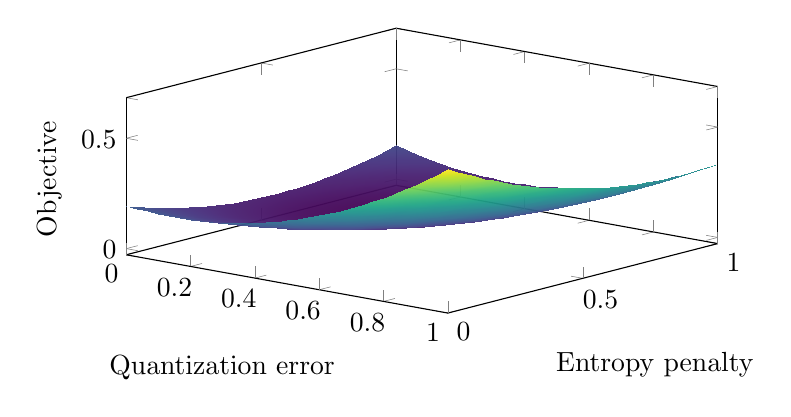
\begin{tikzpicture}
        \begin{axis}[
            width=0.75\linewidth,
            height=5.2cm,
            xlabel={Quantization error},
            ylabel={Entropy penalty},
            zlabel={Objective},
            view={40}{30},
            domain=0:1,
            y domain=0:1,
            samples=31,
            samples y=31,
            colormap/viridis
        ]
            \ifdefined\HCode
                \addplot3[surf, shader=flat, opacity=0.95]{0.6*(x-0.35)^2 + 0.4*(y-0.55)^2 + 0.25*x*(1-y)};
            \else
                \addplot3[surf, shader=interp, opacity=0.95]{0.6*(x-0.35)^2 + 0.4*(y-0.55)^2 + 0.25*x*(1-y)};
            \fi
        \end{axis}
    \end{tikzpicture}
    % Avoid inline math in captions; it wraps poorly in some EPUB renderers.
    \caption{Schematic: Quantization error combined with an entropy-style regularizer (modern SOM variant; for example, a negative sum of p log p over unit usage). Valleys arise when prototypes cover the space evenly; ridges highlight collapse or poor topological preservation.}
    \label{fig:lec5-crossentropy}
\end{figure}

\paragraph{Quantization vs. topographic error.} Given data points \(\{\mathbf{x}_i\}\) and best-matching units \(b_i = \operatorname{BMU}(\mathbf{x}_i)\), the \emph{quantization error} is
\[
    \text{QE} = \frac{1}{N}\sum_{i=1}^N \bigl\|\mathbf{x}_i - \mathbf{w}_{b_i}\bigr\|_2,
\]
which measures reconstruction fidelity. The \emph{topographic error} is the fraction of inputs whose first- and second-best BMUs are not adjacent on the lattice (default: 4-neighbor connectivity), capturing topology preservation. Both metrics reappear in later figures; we monitor QE for representation quality and TE for magnification distortions.

\begin{tcolorbox}[summarybox,title={Batch SOM in practice},breakable]
Online SOM updates one sample at a time: pick a best-matching unit (BMU), nudge it and its neighbors, move on. Batch SOM instead aggregates responsibilities across a dataset (or mini\hyp{}batch) before shifting prototypes:
\begin{align*}
h_{j,i}(t) &= \kappa\big(\text{dist}(j,b(i)); \sigma_t\big),\\
\mathbf{w}_j^{(t+1)} &= \frac{\sum_i h_{j,i}(t)\,\mathbf{x}_i}{\sum_i h_{j,i}(t)}.
\end{align*}
Key differences:
\begin{itemize}
    \item \textbf{Deterministic passes.} Batch updates remove stochastic noise and converge in fewer epochs on static datasets, making results reproducible (useful for dashboards/visual analytics).
    \item \textbf{Parallelism.} Computations collapse to matrix ops (compute BMUs, accumulate weighted sums), so GPUs/CPUs can process large mini\hyp{}batches efficiently.
    \item \textbf{Streaming trade-off.} Online updates remain preferable when data arrive continuously or when you need the map to adapt mid-stream; batch SOM suits offline datasets.
\end{itemize}
Most modern SOM libraries expose both modes, so choose the update rule that matches your data pipeline and stability requirements.
\end{tcolorbox}

\paragraph{Stopping criteria.} Because stochastic updates can eventually increase topographic error, it is standard to stop training once a moving-average validation curve plateaus. \Cref{fig:lec5-early-stopping} shows the canonical trend: fast initial improvement followed by saturation.

\begin{figure}[t]
    \centering
    \begin{tikzpicture}
        \begin{axis}[
            width=0.82\linewidth,
            height=5cm,
            xlabel={Epoch},
            ylabel={Error},
            xmin=0, xmax=60,
            ymin=0, ymax=1,
            legend style={at={(0.5,1.03)},anchor=south,legend columns=2}
        ]
            \addplot[cbBlue, thick, smooth] table {
                epoch quant
                0 0.95
                5 0.78
                10 0.6
                15 0.48
                20 0.39
                25 0.33
                30 0.29
                35 0.27
                40 0.26
                45 0.26
                50 0.27
                55 0.29
                60 0.32
            };
            \addlegendentry{Quantization error}
            \addplot[cbOrange, thick, smooth, dashed] table {
                epoch topo
                0 0.9
                5 0.72
                10 0.55
                15 0.43
                20 0.35
                25 0.3
                30 0.27
                35 0.25
                40 0.245
                45 0.245
                50 0.25
                55 0.27
                60 0.3
            };
            \addlegendentry{Topographic error}
            \addplot[cbPink, very thick, domain=0:60]{0.25} node[pos=0.62, anchor=south west, font=\scriptsize, text=cbPink]{stop window};
        \end{axis}
    \end{tikzpicture}
    \caption{Schematic: Validation curves used to identify an early\hyp{}stopping knee. When both quantization and topographic errors flatten (shaded band), further training risks map drift.}
    \label{fig:lec5-early-stopping}
\end{figure}

\subsection{Limitations of Winner-Takes-All and Motivation for Cooperation}
\label{sec:som_limitations_of_winner_takes_all_and_motivation_for_cooperation}

While WTA is simple and effective for clustering, it has some limitations:
\begin{itemize}
    \item Only one neuron updates per input, which can lead to slow convergence.
    \item The hard competition ignores relationships among neighboring neurons.
    \item The resulting clusters correspond to hard assignments, so boundaries between codebook vectors are sharp with little smoothing across neighboring neurons.
\end{itemize}
The geometric effect of these limitations is easiest to see in \Cref{fig:lec5-softmax-regions}: the left panel shows the brittle Voronoi partitions created by a strict winner-takes-all rule, whereas the right panel demonstrates how shrinking the neighborhood kernel produces softer responsibilities and smoother maps.

\pgfmathdeclarefunction{somindex}{2}{%
    \pgfmathsetmacro{\da}{(#1-0.2)^2 + (#2-0.2)^2}%
    \pgfmathsetmacro{\db}{(#1-0.8)^2 + (#2-0.25)^2}%
    \pgfmathsetmacro{\dc}{(#1-0.28)^2 + (#2-0.78)^2}%
    \pgfmathsetmacro{\dd}{(#1-0.78)^2 + (#2-0.78)^2}%
    \pgfmathparse{%
        (\da<=\db) && (\da<=\dc) && (\da<=\dd) ? 0 :
        ((\db<=\da) && (\db<=\dc) && (\db<=\dd) ? 1 :
        ((\dc<=\da) && (\dc<=\db) && (\dc<=\dd) ? 2 : 3))}%
}
\pgfmathdeclarefunction{somsoftpeak}{2}{%
    \pgfmathsetmacro{\beta}{8}%
    \pgfmathsetmacro{\ta}{exp(-\beta*((#1-0.2)^2 + (#2-0.2)^2))}%
    \pgfmathsetmacro{\tb}{exp(-\beta*((#1-0.8)^2 + (#2-0.25)^2))}%
    \pgfmathsetmacro{\tc}{exp(-\beta*((#1-0.28)^2 + (#2-0.78)^2))}%
    \pgfmathsetmacro{\td}{exp(-\beta*((#1-0.78)^2 + (#2-0.78)^2))}%
    \pgfmathsetmacro{\sumw}{\ta+\tb+\tc+\td}%
    \pgfmathsetmacro{\maxw}{max(max(\ta,\tb),max(\tc,\td))}%
    \pgfmathparse{\maxw/\sumw}%
}
\pgfplotsset{colormap={somregions}{
        color(0cm)=(cbBlue);
        color(0.33cm)=(cbOrange);
        color(0.66cm)=(cbGreen);
        color(1cm)=(cbPink)
}}
\begin{figure}[t]
    \centering
    \begin{tikzpicture}
        \begin{groupplot}[
            group style={group size=2 by 1, horizontal sep=1.1cm},
            width=0.4\linewidth,
            height=0.42\linewidth,
            xmin=0, xmax=1,
            ymin=0, ymax=1,
            xlabel={$x_1$},
            ylabel={$x_2$},
            axis on top,
            enlargelimits=false
        ]
            \nextgroupplot[
                title={Hard BMU regions},
                view={0}{90},
                colorbar style={title={Prototype}, yshift=-2ex},
                zmin=0, zmax=3,
                colormap name=somregions,
                ticks=none
            ]
                \addplot3[surf,shader=flat,point meta=rawz,
                    domain=0:1, y domain=0:1, samples=45, samples y=45]
                    {somindex(x,y)};
                \addplot+[only marks, mark=*, mark size=1.8pt, color=cbBlue] coordinates {(0.2,0.2)};
                \addplot+[only marks, mark=*, mark size=1.8pt, color=cbOrange] coordinates {(0.8,0.25)};
                \addplot+[only marks, mark=*, mark size=1.8pt, color=cbGreen] coordinates {(0.28,0.78)};
                \addplot+[only marks, mark=*, mark size=1.8pt, color=cbPink] coordinates {(0.78,0.78)};
                \node[font=\scriptsize, anchor=west, cbBlue] at (axis cs:0.22,0.22){$r_1$};
                \node[font=\scriptsize, anchor=west, cbOrange] at (axis cs:0.82,0.25){$r_2$};
                \node[font=\scriptsize, anchor=south west, cbGreen] at (axis cs:0.3,0.82){$r_3$};
                \node[font=\scriptsize, anchor=south east, cbPink] at (axis cs:0.78,0.82){$r_4$};
            \nextgroupplot[
                title={Soft assignments},
                view={0}{90},
                colormap/viridis,
                colorbar style={title={Max softmax prob}, yshift=-2ex},
                ticks=none
            ]
                \addplot3[surf,shader=flat,point meta=rawz,
                    domain=0:1, y domain=0:1, samples=45, samples y=45]
                    {somsoftpeak(x,y)};
                \addplot+[only marks, mark=*, mark size=1.8pt, color=black, fill=white] coordinates {(0.2,0.2)(0.8,0.25)(0.28,0.78)(0.78,0.78)};
                \node[font=\scriptsize,anchor=south east,fill=white,inner sep=1pt] at (axis cs:0.98,0.05){$\sigma(t)\ \text{small}$};
            \end{groupplot}
    \end{tikzpicture}
    \caption{Schematic: Voronoi-like regions induced by SOM prototypes (left) and the corresponding softmax confidence after shrinking the neighborhood kernel (right). Softer updates blur the decision frontiers and reduce jagged mappings between adjacent neurons.}
    \label{fig:lec5-softmax-regions}
\end{figure}

To address these issues, the concept of \emph{cooperation} among neurons is introduced. Instead of a single winner neuron updating its weights, a neighborhood of neurons around the winner also update their weights, albeit to a lesser extent. This idea leads to smoother mappings and better topological ordering.

\subsection{Cooperation in Competitive Learning}
\label{sec:som_neighborhood}

\paragraph{Neighborhood Concept}

Consider the output layer arranged in a 2D grid (or lattice) of neurons. For each input \(\mathbf{x}\), after determining the winning neuron \(c\), we define a neighborhood \(\mathcal{N}(c)\) consisting of neurons close to \(c\) in the output space. In practice the neighborhood weight is supplied by the kernel \(h_{jc}(t)\) of \eqref{eq:gaussian_neighborhood_short}, which is positive for units inside the neighborhood (and decays with the lattice distance \(\|\mathbf{r}_j - \mathbf{r}_c\|\)) and zero for units far away.

The neighborhood size typically shrinks over time during training, starting large to encourage global ordering and gradually reducing to fine-tune local details.

\paragraph{Weight Update with Neighborhood Cooperation} The lattice structure and how the best matching unit (BMU) influences nearby neurons are visualized in \cref{fig:lec5-som-lattice-umatrix}. The U-Matrix on the right provides a quick diagnostic for cluster boundaries during training.

\begin{figure}[t]
    \centering
    \begin{tikzpicture}[scale=0.9]
        % Left panel: lattice
        \begin{scope}
            % draw grid of neurons
            \foreach \i in {0,...,4} {
                \foreach \j in {0,...,4} {
                    \filldraw[fill=white, draw=gray!60] (\i,\j) circle (2.2pt);
                }
            }
            % BMU and neighbors
            \filldraw[fill=cbBlue, draw=cbBlue] (2,2) circle (2.4pt);
            \foreach \p in {(1,2),(3,2),(2,1),(2,3),(1,1),(1,3),(3,1),(3,3)} {
                \filldraw[fill=cbGreen!60, draw=cbGreen!60] \p circle (2.2pt);
            }
            \draw[cbBlue, thick] (2,2) circle (1.2);
            % lattice distance scale (one-step neighbor)
            \draw[<->,gray!70] (2,2.2) -- (3,2.2);
            \node[font=\scriptsize,gray!70] at (2.5,2.45) {$\|\mathbf{r}_j-\mathbf{r}_c\|=1$};
            \node at (2,-0.5) {$\mathbf{r}_c$};
            \node[align=center] at (2,-1.1) {SOM lattice and BMU neighborhood};
        \end{scope}

        % Right panel: U-Matrix (toy heatmap; colored but grayscale-friendly)
        \begin{scope}[shift={(7,0)}]
            \begin{axis}[
                width=0.40\linewidth,
                height=0.40\linewidth,
                view={0}{90},
                xmin=-0.5, xmax=4.5,
                ymin=-0.5, ymax=4.5,
                xtick=\empty, ytick=\empty,
                axis lines=none,
                colormap/viridis,
                point meta min=0.30,
                point meta max=0.90,
                colorbar,
                colorbar style={
                    title={avg.\ distance},
                    ytick={0.30,0.60,0.90},
                    yticklabel style={font=\scriptsize},
                    title style={font=\scriptsize},
                },
                title={U-Matrix (neighbor distances)},
                title style={font=\scriptsize},
            ]
                \addplot[
                    matrix plot*,
                    mesh/cols=5,
                    mesh/rows=5,
                    point meta=explicit,
                ] table [meta=z] {
                    x y z
                    0 4 0.85
                    1 4 0.65
                    2 4 0.60
                    3 4 0.70
                    4 4 0.90
                    0 3 0.75
                    1 3 0.55
                    2 3 0.50
                    3 3 0.65
                    4 3 0.85
                    0 2 0.70
                    1 2 0.55
                    2 2 0.45
                    3 2 0.60
                    4 2 0.80
                    0 1 0.65
                    1 1 0.35
                    2 1 0.30
                    3 1 0.40
                    4 1 0.70
                    0 0 0.80
                    1 0 0.60
                    2 0 0.55
                    3 0 0.60
                    4 0 0.85
                };
            \end{axis}
        \end{scope}
    \end{tikzpicture}
    % Avoid inline math in captions; it wraps poorly in some EPUB renderers.
    \caption{Schematic: Left: a 5-by-5 SOM lattice with best matching unit (blue) and neighbors within the Gaussian-kernel radius (green). Right: a toy U-Matrix (colormap chosen to remain interpretable in grayscale) showing average distances between neighboring codebook vectors; higher distances indicate likely cluster boundaries.}
    \label{fig:lec5-som-lattice-umatrix}
\end{figure}

\begin{figure}[t]
    \centering
            \begin{tikzpicture}
                    \begin{groupplot}[
                        group style={group size=3 by 1, horizontal sep=0.55cm},
                        width=0.30\linewidth,
                        height=0.30\linewidth,
                        view={0}{90},
                        xmin=-0.5,xmax=4.5,
                        ymin=-0.5,ymax=4.5,
                        xtick=\empty, ytick=\empty,
                        colormap/viridis,
                        point meta min=0,
                        point meta max=0.7,
                        nodes near coords,
                        nodes near coords style={font=\scriptsize},
                        every node near coord/.append style={fill=white, fill opacity=0.8, text opacity=1, inner sep=0.6pt},
                        mesh/check=false
                    ]
                \nextgroupplot[title={Plane: pixel 1}]
                    \addplot[matrix plot*, mesh/cols=5, mesh/rows=5, point meta=explicit] table [meta=z] {
                        x y z
                        0 0 0.2
                    1 0 0.3
                    2 0 0.4
                    3 0 0.6
                    4 0 0.7
                    0 1 0.1
                    1 1 0.2
                    2 1 0.3
                    3 1 0.5
                    4 1 0.6
                    0 2 0.0
                    1 2 0.1
                    2 2 0.2
                    3 2 0.4
                    4 2 0.5
                    0 3 0.0
                    1 3 0.1
                    2 3 0.2
                    3 3 0.3
                    4 3 0.4
                    0 4 0.0
                    1 4 0.1
                    2 4 0.1
                    3 4 0.2
                        4 4 0.3
                    };
                \nextgroupplot[title={Plane: pixel 2}]
                    \addplot[matrix plot*, mesh/cols=5, mesh/rows=5, point meta=explicit] table [meta=z] {
                        x y z
                        0 0 0.7
                    1 0 0.5
                    2 0 0.4
                    3 0 0.3
                    4 0 0.2
                    0 1 0.6
                    1 1 0.4
                    2 1 0.3
                    3 1 0.2
                    4 1 0.1
                    0 2 0.5
                    1 2 0.3
                    2 2 0.2
                    3 2 0.1
                    4 2 0.0
                    0 3 0.4
                    1 3 0.2
                    2 3 0.1
                    3 3 0.0
                    4 3 0.0
                    0 4 0.3
                    1 4 0.1
                    2 4 0.0
                    3 4 0.0
                        4 4 0.0
                    };
                \nextgroupplot[
                        title={Plane: pixel 3},
                        colorbar,
                        colorbar style={
                            ytick={0,0.35,0.7},
                            yticklabel style={font=\scriptsize},
                        },
                    ]
                    \addplot[matrix plot*, mesh/cols=5, mesh/rows=5, point meta=explicit] table [meta=z] {
                        x y z
                        0 0 0.1
                    1 0 0.2
                    2 0 0.3
                    3 0 0.4
                    4 0 0.5
                    0 1 0.1
                    1 1 0.2
                    2 1 0.3
                    3 1 0.4
                    4 1 0.5
                    0 2 0.1
                    1 2 0.2
                    2 2 0.3
                    3 2 0.4
                    4 2 0.5
                    0 3 0.1
                    1 3 0.2
                    2 3 0.3
                    3 3 0.4
                    4 3 0.5
                    0 4 0.1
                    1 4 0.2
                    2 4 0.3
                    3 4 0.4
                    4 4 0.5
                };
        \end{groupplot}
    \end{tikzpicture}
\caption{Schematic: Component planes for three features on a trained SOM (toy data). Each plane maps one feature's value across the map; aligned bright/dark regions across planes reveal correlated features, complementing the U-Matrix in \Cref{fig:lec5-som-lattice-umatrix}. Interpret brightness comparatively within a plane rather than as an absolute calibrated scale.}
    \label{fig:lec5-som-component-planes}
\end{figure}
The weight update rule generalizes to:
\begin{align}
\mathbf{w}_j(t+1) = \mathbf{w}_j(t) + \alpha(t) \, h_{j c}(t) \left( \mathbf{x} - \mathbf{w}_j(t) \right),
\label{eq:coop_weight_update}
\end{align}
where
\begin{itemize}
    \item \(h_{j c}(t)\) is the \emph{neighborhood function} that quantifies the degree of cooperation between neuron \(j\) and the winner \(c\).
    \item \(\alpha(t)\) is the learning rate at time \(t\).
\end{itemize}

The neighborhood function satisfies:
\[
h_{j c}(t) = \begin{cases}
1, & j = c \\
\in (0,1), & j \in \mathcal{N}(c), j \neq c \\
0, & \text{otherwise}
\end{cases}
\]

\paragraph{Gaussian Neighborhood Function}

A common choice for \(h_{j c}(t)\) is a Gaussian function based on the distance between neurons \(j\) and \(c\) on the output lattice:
\begin{align}
h_{j c}(t) = \exp \left( - \frac{\| \mathbf{r}_j - \mathbf{r}_{c} \|^2}{2 \sigma^2(t)} \right),
\label{eq:gaussian_neighborhood}
\end{align}
where
\begin{itemize}
    \item \(\mathbf{r}_j\) and \(\mathbf{r}_{c}\) are the coordinates of neurons \(j\) and \(c\) on the output grid.
    \item \(\sigma(t)\) is the neighborhood radius (width) at time \(t\), which decreases over training.
\end{itemize}

This function ensures that neurons closer to the winner receive larger updates, while distant neurons are updated less or not at all.

\paragraph{Interpretation}

The cooperative update encourages neighboring neurons to become sensitive to similar inputs, thereby preserving topological relationships in the input space. This is the key principle behind Self-Organizing Maps (SOMs).

\subsection{Example: Neighborhood Update Illustration}
\label{sec:som_example_neighborhood_update_illustration}

Suppose the output neurons are arranged in a 2D lattice as shown schematically in \Cref{fig:som_neighborhood}, where each neuron is indexed by its grid coordinates. For an input \(\mathbf{x}\), neuron \(c\) wins. The neighborhood \(\mathcal{N}(c)\) might include neurons within a radius \(\sigma\) around \(c\).

\begin{figure}[t]
    \centering
    \begin{tikzpicture}[scale=0.8]
        \foreach \x in {0,...,3} {
            \foreach \y in {0,...,3} {
                \node[draw,circle,minimum size=0.5cm,fill=gray!5] (n\x\y) at (\x,\y) {};
            }
        }
        \node[draw,circle,minimum size=0.55cm,fill=cbBlue!40] at (2,1) {};
        \draw[cbGreen, dashed, thick] (2,1) circle (1.5);
        \node at (2,1.5) {\scriptsize BMU $c$};
        \node[cbGreen!70!black] at (3.6,1) {\scriptsize radius $\sigma(t)$};
    \end{tikzpicture}
    \caption{Schematic: SOM lattice with the best-matching unit (BMU) highlighted in blue and a dashed neighborhood radius indicating which prototype vectors receive cooperative updates.}
    \label{fig:som_neighborhood}
\end{figure}

Each neuron \(j\) in \(\mathcal{N}(c)\) updates its weight vector according to \eqref{eq:coop_weight_update}, with the magnitude of update modulated by \(h_{j c}(t)\).

\subsection{Summary of Cooperative Competitive Learning Algorithm}
\label{sec:som_summary_of_cooperative_competitive_learning_algorithm}

\begin{enumerate}
    \item Present an input vector and identify the winning neuron using the discriminant function.
    \item Update the winning neuron's weights and those of its neighbors according to the cooperative rule.
    \item Decrease the learning rate and neighborhood radius according to the annealing schedule.
    \item Repeat for all inputs until the map stabilizes or a maximum number of epochs is reached.
\end{enumerate}
\subsection{Wrapping Up the Kohonen Self-Organizing Map (SOM) Derivations}
\label{sec:som_wrapping_up_the_kohonen_self_organizing_map_som_derivations}

We conclude our derivation and discussion of the Kohonen Self-Organizing Map (SOM) learning algorithm by summarizing the key components and their evolution during training.

Recall the weight update rule for neuron \( j \) at time step \( t \):
\begin{align}
    \Delta \mathbf{w}_j(t) = \alpha(t) \, h_{j,c}(t) \left[ \mathbf{x}(t) - \mathbf{w}_j(t) \right].
    \label{eq:auto:lecture_5_part_i:2}
\end{align}
where:
\begin{itemize}
    \item \(\mathbf{x}(t)\) is the input vector at time \( t \).
    \item \(\mathbf{w}_j(t)\) is the weight vector of neuron \( j \) at time \( t \).
    \item \(c\) is the index of the winning neuron (best matching unit) for input \(\mathbf{x}(t)\).
    \item \(\alpha(t)\) is the learning rate, a monotonically decreasing function of time.
    \item \(h_{j,c}(t)\) is the neighborhood function centered on the winning neuron \( c \), also decreasing over time.
\end{itemize}

\paragraph{Neighborhood Function and Its Role}

The neighborhood function \( h_{j,c}(t) \) typically takes a Gaussian form:
\begin{align}
    h_{j,c}(t) = \exp\left(-\frac{\| \mathbf{r}_j - \mathbf{r}_{c} \|^2}{2\sigma^2(t)}\right).
    \label{eq:neighborhood_function}
\end{align}
where:
\begin{itemize}
    \item \(\mathbf{r}_j\) and \(\mathbf{r}_{c}\) are the positions of neurons \( j \) and \( c \) on the SOM lattice.
    \item \(\sigma(t)\) is the neighborhood radius, which decreases over time.
\end{itemize}

This function ensures that neurons closer to the winning neuron receive larger updates, while those farther away receive smaller or zero updates. Initially, \(\sigma(t)\) is large, allowing broad neighborhood cooperation, but it shrinks as training progresses, focusing updates increasingly on the winning neuron itself.

\paragraph{Time-Dependent Parameters}

Both the learning rate \(\alpha(t)\) and neighborhood radius \(\sigma(t)\) decrease over time, typically following exponential decay laws:
\begin{align}
    \alpha(t) &= \alpha_0 \exp\left(-\frac{t}{\tau_\alpha}\right), \\
    \sigma(t) &= \sigma_0 \exp\left(-\frac{t}{\tau_\sigma}\right),
    \label{eq:decay_parameters}
\end{align}
where \(\alpha_0\) and \(\sigma_0\) are initial values, and \(\tau_\alpha, \tau_\sigma\) are time constants controlling the decay rates.

\paragraph{Summary of the Six Learning Steps}
\label{sec:som_training_steps}

SOM training iteratively repeats the following six steps:

\begin{tcolorbox}[summarybox,title={Self-Organizing Map (SOM) training pseudocode}]
\begin{enumerate}
    \item \textbf{Initialize} weight vectors \(\mathbf{w}_j(0)\) randomly or from samples.
    \item For iteration \(t=0,\ldots,T\):
    \begin{enumerate}
        \item Sample an input \(\mathbf{x}(t)\).
        \item Find the best matching unit (BMU) \(c = \arg\min_{j} \|\mathbf{x}(t)-\mathbf{w}_j(t)\|_2^2\).
        \item Compute neighborhood coefficients \(h_{j,c}(t)\).
        \item Update every neuron:
        \[
            \mathbf{w}_j(t+1) = \mathbf{w}_j(t) + \alpha(t)\, h_{j,c}(t)\Bigl(\mathbf{x}(t)-\mathbf{w}_j(t)\Bigr).
        \]
        \item Decay learning-rate \(\alpha(t)\) and neighborhood radius \(\sigma(t)\) (e.g., exponentially).
    \end{enumerate}
\end{enumerate}
\end{tcolorbox}

\begin{tcolorbox}[summarybox,title={Batch SOM (deterministic pass)}]
\begin{enumerate}
    \item Fix centers \(\mathbf{r}_j\) on the lattice; initialize \(\mathbf{w}_j\) (random data or along PCA directions).
    \item Repeat until convergence or max epochs:
    \begin{enumerate}
        \item Assign each \(\mathbf{x}_n\) to its BMU \(c_n\).
        \item For each neuron \(j\), update
        \[
        \mathbf{w}_j \leftarrow \frac{\sum_n h_{j,c_n}(t)\,\mathbf{x}_n}{\sum_n h_{j,c_n}(t)}.
        \]
        \item Decay \(\alpha(t),\sigma(t)\).
    \end{enumerate}
\end{enumerate}
Batch SOM (one pass per epoch) is deterministic given the assignments; it often stabilises faster than purely online updates.
\end{tcolorbox}

\noindent These procedural steps implement three conceptual \emph{stages}: (1) \textbf{Initialization} (seed the weight lattice), (2) \textbf{Competition} (select the best-matching unit for each input), and (3) \textbf{Cooperation} (neighborhood-weighted updates plus the associated parameter decay). Calling out these stages separately helps when comparing SOMs to other competitive-learning algorithms later in the chapter.

These steps are repeated until convergence criteria are met, such as a maximum number of iterations or a threshold on weight changes.

\paragraph{Stages vs. Steps}

It is important to distinguish between the \emph{three stages} of SOM learning and the \emph{six steps} described above:

\begin{itemize}
    \item \textbf{Stages:}
    \begin{enumerate}
    \item \emph{Initialization:} setting up the network.
    \item \emph{Competition:} neurons compete to respond to input.
    \item \emph{Cooperation:} neighboring neurons cooperate to update weights.
    \end{enumerate}
    \item \textbf{Steps:} The six procedural steps in \Cref{sec:som_training_steps} that operationalize these stages during training.
\end{itemize}

\subsection{Applications of Kohonen Self-Organizing Maps}
\label{sec:som_applications_of_kohonen_self_organizing_maps}

Kohonen SOMs are widely used for:

\begin{itemize}
    \item \textbf{Clustering:} Grouping similar data points without supervision.
    \item \textbf{Dimensionality Reduction:} Mapping high-dimensional data onto a low-dimensional space (often arranged as a discrete lattice in SOM implementations) for visualization and exploratory analysis.
    \item \textbf{Data Visualization:} Providing intuitive heatmaps or component planes that reveal correlations and patterns across features.
\end{itemize}

\paragraph{Relation to k-means and modern variants}

When the SOM lattice is collapsed to a single point, the algorithm reduces to a k-means-style prototype update without any notion of neighborhood \citep{MacQueen1967}; SOMs therefore sit between pure clustering (k-means) and manifold learning, adding a topographic prior that encourages neighboring units to represent similar inputs. Recent ``neural-SOM'' hybrids embed SOM-like updates inside deep networks, but still rely on the same BMU search and neighborhood-weighted updates described above.

\begin{tcolorbox}[summarybox,title={Theory notes and recipes}]
\textbf{Convergence/magnification:} With decays \(\alpha(t)\to 0\), \(\sigma(t)\to 0\) and \(\sum_t \alpha(t)=\infty\), \(\sum_t \alpha^2(t)<\infty\), SOM updates converge under mild assumptions \citep{ErwinObermayerSchulten1992,CottrellFort1986}. Lattice density follows data density (magnification) so dense regions attract more neurons.\\
\textbf{Map-size/schedule recipe:} Use \(5\sqrt{N}\)--\(10\sqrt{N}\) neurons when unsure; hex grids reduce anisotropy; toroidal lattices mitigate edges. Initialize \(\mathbf{w}_j\) from data or first two PCs; \(\alpha_0\in[0.1,0.5]\to \alpha_{\min}\approx 10^{-3}\); \(\sigma_0\) equal to the map radius, decaying to 1--1.5 cells.
\end{tcolorbox}

\begin{tcolorbox}[summarybox,title={Related and growing variants}]
\textbf{Neural Gas / Growing Neural Gas} \citep{MartinetzBerkovichSchulten1993,Fritzke1994GrowingNeuralGas} drop the fixed lattice and learn topology or add units dynamically. \textbf{GTM} (Bishop et al.) provides a probabilistic, topographic embedding with likelihoods/uncertainty. SOMs sit between k-means (no topology) and these adaptive-topology models.
\end{tcolorbox}

\paragraph{Complexity and out-of-sample mapping.} A full online epoch costs \(O(NM)\) (N data, M units); batch passes cost similar but fewer epochs. For large M, use approximate nearest-neighbor BMU search (k-d trees, FAISS). New points map via their BMU; optional soft responsibilities use \(h_{ci}\) for smoothing.
\paragraph{Theory link to other chapters.} SOMs learn prototypes like the centers in \Cref{chap:rbf} but add a topographic prior; quality diagnostics (QE/TE) can be tracked with the validation-curve diagnostics in \Cref{chap:supervised}. For task-driven embeddings, see \Cref{chap:cnn,chap:nlp}; Hopfield (\Cref{chap:hopfield}) contrasts with energy-based associative recall.

\paragraph{Quality measures and magnification.} Two diagnostics are standard when reporting SOM quality:
\begin{itemize}
    \item \textbf{Quantization error (QE):} average Euclidean distance between each input and its BMU. Lower QE indicates prototypes that better represent the data manifold.
    \item \textbf{Topographic error (TE):} fraction of inputs whose first- and second-best BMUs are not adjacent, quantifying topology preservation (magnification factor).
\end{itemize}
Tracking both metrics reveals whether the neighborhood decay is too slow (over-smoothing) or too aggressive (tearing the topology). \Cref{chap:supervised}'s learning-curve plots suggest early\hyp{}stopping heuristics: stop when QE/TE on a validation split flatten.

\begin{tcolorbox}[summarybox,title={Key takeaways}]
\begin{itemize}
    \item SOMs perform topology-preserving vector quantization on a discrete lattice.
    \item A shrinking neighborhood and decaying learning rate drive coarse-to-fine organization.
    \item U-Matrices and quantization/topographic errors are practical diagnostics for convergence.
\end{itemize}

\medskip
\noindent\textbf{Minimum viable mastery.}
\begin{itemize}
    \item Given \(x\), compute the BMU, write the weight update \(w_i \leftarrow w_i + \alpha(t) h_{ci}(t) (x-w_i)\), and explain how \(h_{ci}\) enforces cooperation.
    \item Interpret a U-Matrix and component planes as diagnostics for neighborhood structure and convergence.
    \item Choose sensible \(\alpha(t)\) and \(\sigma(t)\) schedules and justify them using QE/TE validation curves.
\end{itemize}

\noindent\textbf{Common pitfalls.}
\begin{itemize}
    \item Using a map that is too small or a neighborhood decay that is too aggressive (tearing the topology).
    \item Skipping input normalization, causing prototypes to track scale rather than structure.
    \item Treating lattice distance as a true metric in data space (SOM topology is approximate, not exact geometry).
    \item Over-interpreting a single run without checking QE/TE plateaus and sensitivity to initialization.
\end{itemize}
\end{tcolorbox}

\begin{tcolorbox}[summarybox,title={Exercises and lab ideas}]
\begin{itemize}
    \item Train a \(10\times 10\) SOM on handwritten digits (MNIST) and plot component planes; report quantization/topographic errors as training progresses.
    \item Implement the six-step SOM procedure with both Gaussian and rectangular neighborhood functions and compare convergence speed.
    \item Visualize the effect of annealing schedules by freezing the learning rate and neighborhood radius at different epochs and observing the resulting U-Matrix.
    \item Compare SOM prototypes to K-means centers on the same dataset; sweep \((\sigma(t))\) schedules and map sizes; report QE/TE and a trustworthiness@k measure.
\end{itemize}

\medskip
\noindent\textbf{If you are skipping ahead.} Keep the notion of an ``energy landscape'' from this chapter in mind: \Cref{chap:hopfield} makes that idea explicit with a Lyapunov energy, and later attention models (\Cref{chap:transformers}) can be read as learned, content-based neighborhood selection.
\end{tcolorbox}

\medskip
\paragraph{Where we head next.} \Cref{chap:hopfield} extends the unsupervised theme by studying Hopfield networks, energy-based models that complement SOMs with associative memory dynamics and pave the way for modern attention mechanisms.

\paragraph{References.} Full citations for works mentioned in this chapter appear in the book-wide bibliography.
